\documentclass{article}


%\usepackage{nips_2018}
\usepackage[final]{nips_2018}

\usepackage[utf8]{inputenc} % allow utf-8 input
\usepackage[T1]{fontenc}    % use 8-bit T1 fonts
\usepackage{hyperref}       % hyperlinks
\usepackage{url}            % simple URL typesetting
\usepackage{booktabs}       % professional-quality tables
\usepackage{amsfonts}       % blackboard math symbols
\usepackage{nicefrac}       % compact symbols for 1/2, etc.
\usepackage{microtype}      % microtypography

\usepackage{graphicx}
\usepackage{tabularx}

\usepackage{multicol}
\usepackage{lipsum}    
\usepackage{mwe}


% Python syntax highlighting like Jupyter Notebook
\usepackage{minted}







\title{Approximating the Music taste of Andreas Lindholm (DRAFT)}

\author{
submission ID S730
}



\begin{document}
    \maketitle
    kvar att göra och inkorporera

1) Snacka om komplexitet av olika soters nnär man väljer rätt metod att säta i produktion.  Tänk hur allt skulle skala om man ökasr antal features, låtar, användare. Basically: en metod med enstka aprocent sämmree accuracy men lätt/billigt att tränna är bättre än att en "dyr" metod. 

2.) i edvins figure med ytplott - Mention that that all surface ploots looked similar across dpreprocesing data sets was a common phomonen. Använd dessa figureer som typ exempel av andra försök att tweaka hyper parameter.


3) alla skriver i method delen sin model och hur ni tweaka hyperparamterna. tänk på följande: 

2) Aconcisedescriptionofeachoftheconsideredmethods,andhowtheyareappliedtotheproblem. Even if you used high-level commands, such as glm() for logistic regression, you should explain what is ‘under the hood’ of the command! Please, use your own words. We already know what is written in the book and on Wikipedia, so do not copy-paste from there. Writing concise summaries are for your own learning, and their quality is crucial to obtain a gold star.

4) ta med naive bayes i performance tabellen. 

    \begin{abstract}
    The problem of statistical learning has many use cases and lie as the foundation for machine learning problems. A general use case for statistical learning is, from data, determine attributes of future data or even predict future data point values. Problems are categorized into quantitative and qualitative problems or regression and classification problems. 
    In this paper, we are using classification algorithms on a data set of songs favored by our teacher, Andreas Lindholm, with the aim of classifying more songs to his liking. The final section of this paper also discusses the ethical aspects of this.
    
    
    msummerixe which methods where worst and best,  
    \end{abstract}
    
    \section{Introduction}
    A persons taste in music is often times very particular and highly individual. What one individual enjoys is often very varied and sometimes difficult to subjectively describe and quantify. Most often, it boils down to either 'liking' a song or 'not'. Given this simplified 'like' or 'dislike' labeling of songs heard, what is interesting from a machine learning perspective is the ability to model and predict a persons preference for a song based on knowledge from a set of previous liked and disliked songs. More concretely, for a given data set $ D = \big( \mathbf{x_i}, y_{i} \big) ^N $ where $\mathbf{x_i}$ is some feature vector representing a song and $y_i$ being the corresponding 'like' / 'dislike' class label. If we let the function $f$ represent a persons "song preference function" with $ f(\mathbf{x_i})$ being their 'like'/'dislike' preference of song $x_i$, then the aim of being able to predict the music taste of said person is essentially that of training a model $ \hat{f}$ such that $ \hat{f}(\mathbf{x_i})$ approximates $ f(\mathbf{x_i})$ over 'all' possible songs. In this project, our aim was to select, train and evaluate classification algorithms from five different families of statistical learning models in order to predict the song preferences of Docent Andreas Lindholm. 
    
    The models chosen and evaluated were logistic regression (regression family), Random forests & Gradient booted trees. (decision tree family), Naive Bayes (Baysian inference family), k-Nearest Neighbor and SVM.
    
    The data set used to train the models consists of 750 songs with the target label of either liked ('1') or disliked ('0'). Each song in the data set has a feature vector of 13 attributes that describe high level characteristics. See [1] for a more detailed description of each attribute. Of the 13 features three were categorical('mode', 'key' and 'time\_signiture' ), while the rest ('acousticness', 'danceability', 'duration' ,'energy', 'speechiness', 'tempo', 'valence',  'instrumentalness', 'liveness' and 'loudness') were numerical. 
    All models used are implemented and tweaked using python and the scikit learn library. 
   
   
   
   
    % Methods and model
    \section{Models \& Method}
    In this section we will mention our initial exploratory data analysis approach as well as our method choice for selecting, implementing, training, optimizing evaluating the chosen classifiers. 
    
    \subsection{Initial exploratory Data analysis, Scaling & Feature selection}
    
    The initial data exploration phase began with a preliminary pair plotting of all-against-all features to get an initial "feel" for the data. We next scaled our data set using Z-score scaling of numerical continuous features. The transformation of each value given by  
    % Equation    
   \[ x \leftarrow \frac{x-\mu_{feature} }{s_{feature}}\]
   
   Scaling was done for downstream analysis when we train our chosen models. Scaling data  makes some models perform much better when all features are within the same value range, reducing wide sensitivity for features that span differently large scales. Not scaling specially affects performance for models that involve distance measures between data points (e.i. kNN, SVM and other distance based classifier). Next, a correlation matrix was computed (including the target feature 'label'), which we used to drop features that had near zero correlation with the 'label'. From these, two new data set were obtained - data sets between 5 and 10 features in term of highest absolute value of correlation. The type of scalar was determined empirically. 
   
   
   
   
   % Models and tuning
    \subsection{Models and tuning}
    
    When estimating a model, there is always a trade-off describing a models generalized error, steaming from statistics as the sum of three interlinked different errors: 
    \textit{(1) Bias: } The Generalized error due to incorrect assumptions, such as predicting the data to be linear when it is quadratic. High-bias models is most likely to under-fit the data.
    \textit{(2) Variance: }Error due to a models sensitivity due to small variations in the training data. A model with high degrees of freedom is likely to have a high variance, resulting in over-fitting the data.
    \textbit{(3) Irreducible error: } Error due to inherent noise in the data. This error can only be reduced by collecting new data and or cleaning up the data, such as out-liers, features with no contribution and so on. [2]
        
    
    
    
    
    
    
    
    We split the data into three parts. Training-, validation- and test set in the ratio 90-10, with a cross-validation of 10-folds used to check the average mean performance measure for each tested model in the training set. The choice of which model to use in a hypothetical "in production use" is based not only on the performance but also, model complexity.
    

    Mention that we used and trained four types models from four model families. The predictive performance of all five models where compared not only between themselves, but also between a base-line "Always predict/classify as "Like"). When finally proposing which one to choose "enterprise product" 



    The following describes the method specific training and tuning procedures: 
    
    
    \\
    LÄGG TILL KORTFATTAT HUR DEN KLASSIFISERAR OCH VAD HYPERPARAMETRARNA GÖR
    
    \textit{Logistic regression:} asdasd
    \textit{Naive Bayes} MARKUS SKRIVER DÄR SEDAN
    \textit{Random forest:} classifiers was trained on four training sets, one Min-Max scaling using sckikit-learns built-in function.
    
    Hyperparamters tuned were tree depth (from 1 to 10 nodes deep) and the number of trees, ranging from 1-10 and 50-450 respectively.
    
    \textit{Gradient Boosting Classifier:}
    A Decision Tree based Boosting classifier. Parameters chosen for tuning was subsample size and number of base classifiers. Subsample size ranged from 0.5 to 1 and number of base classifiers from 10 to 100.
    
     I focused on tuning two paramaters to make them easier to visualize, for RandomForest Depth and number of Trees were tuned and for GradientBoost subsample size and number of sequential classifiers.
    
    These were chosen becuase they have large impact on the bias-variance trade-off and should be educational to investigate.

    
    \textit{support vector machine} 
    
    \textit{k-Nearest Neighbor}
    - optimized for selected features and for k
    
    \subsection{Evaluation and selection}
    

    
    \section{Results}
    %Mean cross-validation score was use to evaluate feature predictions such as the importance for scaling.
    %Using kNN classifier, as a base classifier, the min-max scaling was chosen empirically because of its score (0.78) against standard/z-score scaling (0.67) and without scaling (057).
    
    %Using the same validation score, 
    \subsection{Data Exploration}

    
    - Reference figure 1 and 2. 
    - 
    
     \begin{figure}
        \centering
        \includegraphics[width=0.6\textwidth]{feature_corr_w_label.png}
        \caption{Correlation values between all features with the target feature 'label'.}
        \label{fig:my_label}
    \end{figure}
    
    
    %\begin{figure}
    %    \centering
    %   \includegraphics[width=0.48\textwidth]{Pos_corr.png}
    %   \includegraphics[width=0.48\textwidth]{neg_corr.png}
    %    \caption{Correlation matrix of features in respective 'label'.}
    %    \label{fig:my_label}
    %\end{figure}
    
    
    
    \begin{figure}
        \centering
        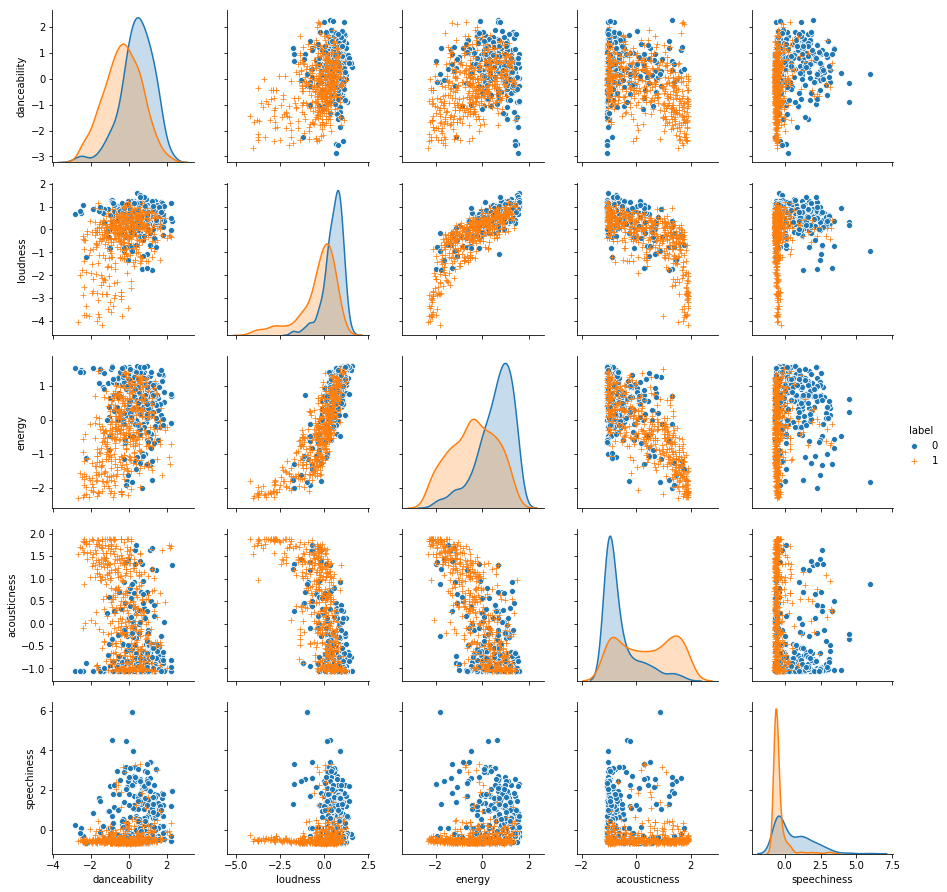
\includegraphics[width=0.8\textwidth]{corr_plot_top_5}
        \caption{Pairwise correlation plots for the top five features with high absolute correlation with 'label'. Blue represents songs liked and orange indicates disliked songs }
        \label{fig:my_label}
    \end{figure}
    
    \subsection{Model Performance}
    


    
    
    
    
    
    \begin{table}[]
        \centering
        \begin{tabular}{c | c | c | c | c | c }
        \hline
          * &  Logistic Regression & Gradient Boosting & Random Forest & kNN  & SVM & \\
        \hline   
           raw  & 0.64770 & 0.83736 & 0.85073 & 2 & 2  \\
         \hline
           scaled all & 0.80537 & 0.84000 & 0.85078 & 2  & 2 \\
            
            min max scaling & 0.81198 & 0.83874 & 0.84939 & 2 & 2 \\
        
           Z scaled top & 0.81202 & 0.84540 & 0.85208 & 2& 2  \\
           
           Z scaled top 10 & 0.81867 & 0.84402 & 0.84669 & 2& 2 \\
        
        \end{tabular}
        \caption{Performance table for each model using 4 types of data pre-processing}
        \label{tab:my_label}
    \end{table}
    
    In Fig.\ref{fig:randfor} we can see the Validation Error yielded by 4 different pre-processed sets of training data. As we can see convergence is reached already at 50 trees and the only thing that affects the Validation Error is increasing the depth of the Tree. It is likely that convergence was reached before 50 Trees. 
    
    \begin{figure*}[ht!]
        \includegraphics[width=.5\textwidth]{randomForest_minmax_allfeatures.png}\hfill
        \includegraphics[width=.5\textwidth]{randomForest_maj_scaling.png}\hfill
        \includegraphics[width=.5\textwidth]{randomForest_maj_scaling_10.png}\hfill
        \includegraphics[width=.5\textwidth]{randomForest_maj_scaling_5.png}\hfill

        \caption{From left to right, top to bottom there the plots are: MinMax Scaling with all features, Z-Scaling(?) with all features, Z-Scaling with the 10 features most correlated with the decision and Z-Scaling with the 5 features most correlated with the decision respectively.} 
            \label{fig:randfor}
    \end{figure*}
        
    Reducing the sample sixe of features selected for making the decision should increase the bias but lower variance, together with increase in number of trees we should be able to find a sweet-spot in the bias-variance trade-off.
        
    \begin{figure*}[ht!]
        \includegraphics[width=.5\textwidth]{GradBoost_raw.png}\hfill
        \includegraphics[width=.5\textwidth]{GradBoost_MinMax.png}\hfill
        \includegraphics[width=.5\textwidth]{GradBoost_Z.png}\hfill
        \includegraphics[width=.5\textwidth]{GradBoost_Z5.png}\hfill
        \includegraphics[width=.5\textwidth]{GradBoost_Z10.png}\hfill

        \caption{Numbered from 1 to 5 are Raw, MinMax-Scaled, Z-Scaled, Z-Scaled with top 5 features and Z-scaled with top 10 features respectively. Top feature is in this case determined by correlation with decision.}
        \label{fig:randfor}
    \end{figure*}
        
    The resulting plot shows that there's no trend in increase of the parameters leading to a better Cross Validation score.
      
      
    \section{Discussions}
    
    - certain models have within them,internal feature selection properties. Such as LASSO and Decion trees. 
    
    - discuss improvements in terms of model but also in terms of the data. More features, even higher level features. 
    
    other approaches. 
    
    %Edvins part:
    The tuning of the ensemble methods yielded very little improvements other than that a stump was worse than a deeper tree when it comes to Random Forest. This is however well in line with the properties of the algorithm as Random forest is a Bagging-derivative and therefore benefits from a low bias-high variance model, such as a deeper tree, and then reducing variance by averaging over many trees. The theory was that Gradient Boosting should have increased the validation error when taking too small subsamples as this increases bias. In return, we could then reduce the bias (and further reduce variance) through increasing the amount of base classifiers. This was not the case however as the validation error remained pretty much constant. This could be due to that the ranges of investigation were chosen somewhat arbitrary and convergence lied outside of that range.
    
    
    
    topics to take into account:
    
    - We seem to have features that are correlated with one another. We see this from figure figure X. Having highly correlated features means that we get little additional information about 
    
    Stuff we could have do more /better: \newline
    
    - ´improved feature selection using LASSO (L1 regularization on Regression) and see investigate the penalization parameter affects the number of features with non zero coefficients. 
    
    \subsection{On the ethics of ML-inference and its use (working title)}
    
    
    Example scenario 1: 
    (make more formal later. )
    Ones music preferences being used as part of the data about a person ensure of state controlled 
    
    
    \\
    \\
    Example scenario 2: 
    A music application with database of music preferences and ability to algorithmically promote or play songs of the user’s preference, and a news application with database the sentiments of articles and of likes, shares and comments.
    
    Music has great power to shape and influence emotions. Consider the director choosing a powerful, epic score for the scene where the heroes triumph, moving the audience to tears, or how Yakety Sax can turn a dreadful sequence of events hilarious. 
    
    Now say the news app is sponsored by party A and a user is reading an article about this party gaining votes on party B in polls while listening to music through the music app in the background, with the “shuffle” option selected. Normally this would play completely random songs from the users library, or maybe algorithmically chosen to represent as diverse a selection of songs from their library as possible, but how can you tell random from purposefully chosen? What if triumphant or happy songs were chosen to be played next while the user read the hypothetical article? Might they not come away from the article feeling slightly more positive towards party A, feeling the party’s triumph as their triumph? What if music the user often skipped, or otherwise showed signs of liking less, was chosen to play next when they read articles about party B’s successes or party A’s failures? Maybe they‘d be more likely to tap away and read something else. Or perhaps the algorithm is designed to favour louder and angrier songs when the user reads about party B’s controversies, prompting the user to share the article or leave angry comments.
    
    Even if the user doesn’t have the “shuffle” option selected, there are still avenues of influence; people prefer louder music, all else being equal. The algorithm could increase the volume of the music slightly when the user reads articles they should feel good about, or introduce slight background noise or change the equalizer to make the music duller when the user should feel worse or unsatisfied with the content of the article they’re reading. 
    
    These tactics might not turn any users’ allegiance from party B to party A, but out of tens of thousands of users reading tens of articles per day over hundreds of days, perhaps the turnout for party A could be increased by a few percentage points and that for party B decreased by a few. 
    
    No user would say yes to the question, “would you like us to subtly influence you through the music you listen to, such that you feel less engaged with the causes you care about, unless they are the ones we approve of?”, so this is clearly not ethical. The core idea though, to influence mood and emotions through context aware music choices could be used for good. A gambling addicted user could permit the app to choose less engaging music whenever the gambling app is open for instance.













\newpage

% Include code
\section*{Appendix}
\begin{minted}{python}
#SMLClassifier.py
import numpy as np
import pandas as pd
from sklearn import *

# Diffrent classifiers
from sklearn.linear_model import LinearRegression  
from sklearn.naive_bayes import GaussianNB
from sklearn.preprocessing import StandardScaler
from sklearn.datasets import make_moons, make_circles, make_classification
from sklearn.neural_network import MLPClassifier
from sklearn.neighbors import KNeighborsClassifier
from sklearn.svm import SVC
from sklearn.gaussian_process import GaussianProcessClassifier
from sklearn.gaussian_process.kernels import RBF
from sklearn.tree import DecisionTreeClassifier
from sklearn.ensemble import RandomForestClassifier, AdaBoostClassifier
from sklearn.naive_bayes import GaussianNB
from sklearn.discriminant_analysis import QuadraticDiscriminantAnalysis

# Process data and handle classsification size and accuracy
from sklearn import preprocessing
#from sklearn.preprocessing import StandardScaler
from sklearn.preprocessing import MinMaxScaler
from sklearn.preprocessing import LabelEncoder
from sklearn.model_selection import train_test_split, cross_val_score
from sklearn.metrics import accuracy_score, confusion_matrix, classification_report
from sklearn.model_selection import StratifiedKFold
import matplotlib.pyplot as plt



# Read data and and data to predict
songs = pd.read_csv('training_data.csv')
songsToClassify = pd.read_csv('songs_to_classify.csv')

# Set the "Label to make predictions agains"
label = songs.label                         
features = songs.drop(columns='label')      
y = label
X = features

# Rescale the data features with min-max for improved accuracy 
# KNN classifier with "Min-Max" =  0.78
sc = MinMaxScaler()
X = sc.fit_transform(X)
songsToClassify = sc.fit_transform(songsToClassify)

# Initialize classifier
"""---------------------- Uncomment to test them: ----------------------"""
clf = KNeighborsClassifier(n_neighbors=5)
#clf = DecisionTreeClassifier(max_depth=5)
#clf = RandomForestClassifier(max_depth=8, n_estimators=5000, max_features=2) 
#clf = GaussianNB()
#clf = LinearRegression()
#clf = QuadraticDiscriminantAnalysis() 
#clf = SVC(gamma=2, C=2)
#clf = KNeighborsClassifier(n_neighbors=15) 
#clf = AdaBoostClassifier()
#clf = MLPClassifier(alpha=0.2)
#clf = QuadraticDiscriminantAnalysis() 




# Use cross_val_score function
# cv=10 for 10 folds
# scoring='accuracy' for evaluation metric
scores = cross_val_score(clf, X, y, cv=10, scoring='accuracy')

print("\nScores from the crossvalidation is: \n", scores)
print("\n\nMedian score from the crossvalidation is: \n", scores.mean())

X_train, X_test, y_train, y_test = train_test_split(X, y, test_size=0.2, random_state=2)

# Train our classifier
model = clf.fit(X_train, y_train)

# Make predictions on test
prediction = clf.predict(X_test)

#Predict the response for test dataset
clf.fit(X, y)
y_pred = clf.predict(X_test)

# Prediction in comparison of the training and test data
print("\n\n\nCurrent accuracy is from predicted values: \n", accuracy_score(y_pred, y_test))
print("\n\nPrecdicted classification from test labels: \n\n", y_pred)

# This is prediction of actual songs liked/displiked
print("\n\n\n == Now the real classification ==\n\n", y_pred)
y_songsToClassifyPred = clf.predict(songsToClassify)

# print(y_songsToClassifyPred)
formatedPrediction = ["".join(item) for item in y_songsToClassifyPred.astype(str)]
formatedPrediction = ''.join(formatedPrediction)

# convert format to string with no spaces
print(formatedPrediction)
\end{minted}











\newpage

%References
\section*{References}
\small

%% New references %%
[1] Spotify API (2019) Get audio features from a track. Spotify, {\it https://developer.spotify.com/documentation/web-api/reference/tracks/get-audio-features/} \ Accessed 04 February 2019

[2] Géron, Aurélien\ (2017) Hands-on machine learning with scikit-learn & Tensorflow.
{\it Concept, tools and techniques to build inteligent systems} first edition, pp.\ 127. O'Reilly, O'Reilly media, Inc





%% OLD %%
[1] Alexander, J.A.\ \& Mozer, M.C.\ (1995) Template-based algorithms
for connectionist rule extraction. In G.\ Tesauro, D.S.\ Touretzky and
T.K.\ Leen (eds.), {\it Advances in Neural Information Processing
  Systems 7}, pp.\ 609--616. Cambridge, MA: MIT Press.

[2] Bower, J.M.\ \& Beeman, D.\ (1995) {\it The Book of GENESIS:
  Exploring Realistic Neural Models with the GEneral NEural SImulation
  System.}  New York: TELOS/Springer--Verlag.

[3] Hasselmo, M.E., Schnell, E.\ \& Barkai, E.\ (1995) Dynamics of
learning and recall at excitatory recurrent synapses and cholinergic
modulation in rat hippocampal region CA3. {\it Journal of
  Neuroscience} {\bf 15}(7):5249-5262.
    
    
    
\end{document}
